% !TEX root = main.tex
\subsubsection{Contextual linear Gaussian bandits: Oracle TS}
\label{sssec:evaluation_contextual_linear_oracle}

% Linear Gaussian results (moved to place them here)
\begin{figure*}[!h]
	% A=2
	\centering
	\begin{subfigure}[b]{0.32\textwidth}
		\centering
		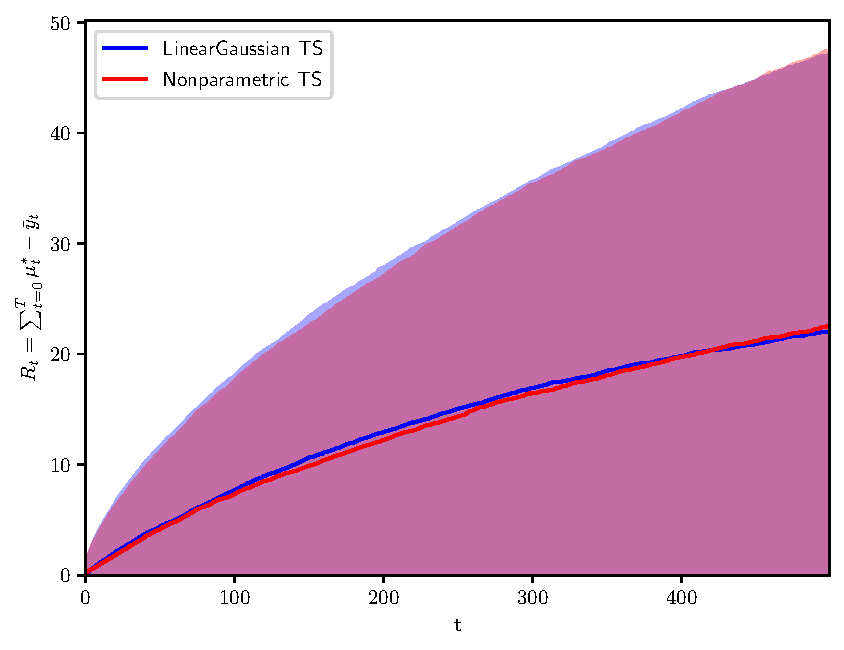
\includegraphics[width=\textwidth]{./figs/linearGaussian/cumregret_A2_-01_-01_01_01_1_1}
		\vspace*{-5ex}
		\caption{$|\mathcal{A}|=2$,\\ \hspace*{0.3cm} $\theta_{0,i}=-0.1$, $\theta_{1,i}=0.1$.}
		\label{fig:linear_gaussian_A2_01}
	\end{subfigure}
	\begin{subfigure}[b]{0.32\textwidth}
		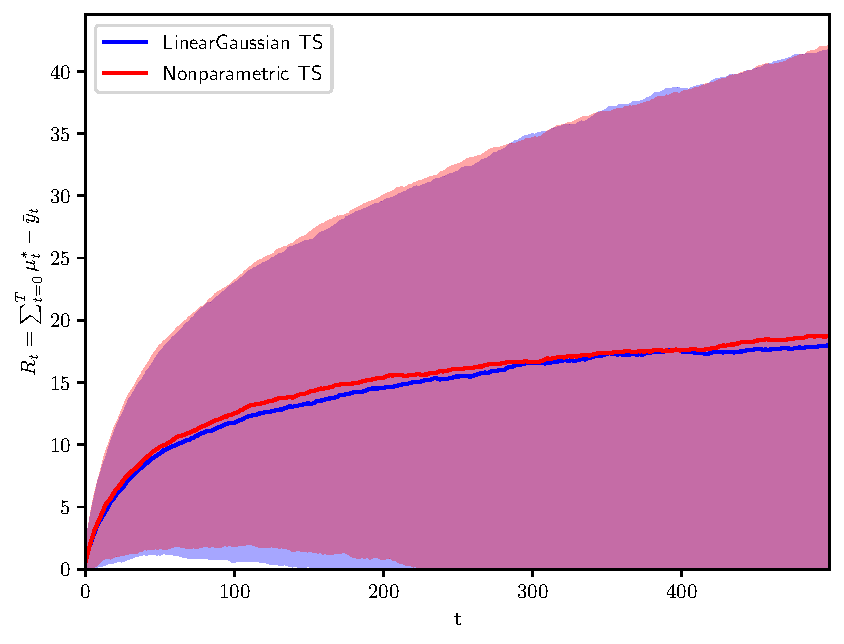
\includegraphics[width=\textwidth]{./figs/linearGaussian/cumregret_A2_-05_-05_05_05_1_1}
		\vspace*{-5ex}
		\caption{$|\mathcal{A}|=2$,\\ \hspace*{0.3cm}  $\theta_{0,i}=-0.5$, $\theta_{1,i}=0.5$.}
		\label{fig:linear_gaussian_A2_05}
	\end{subfigure}
	\begin{subfigure}[b]{0.32\textwidth}
		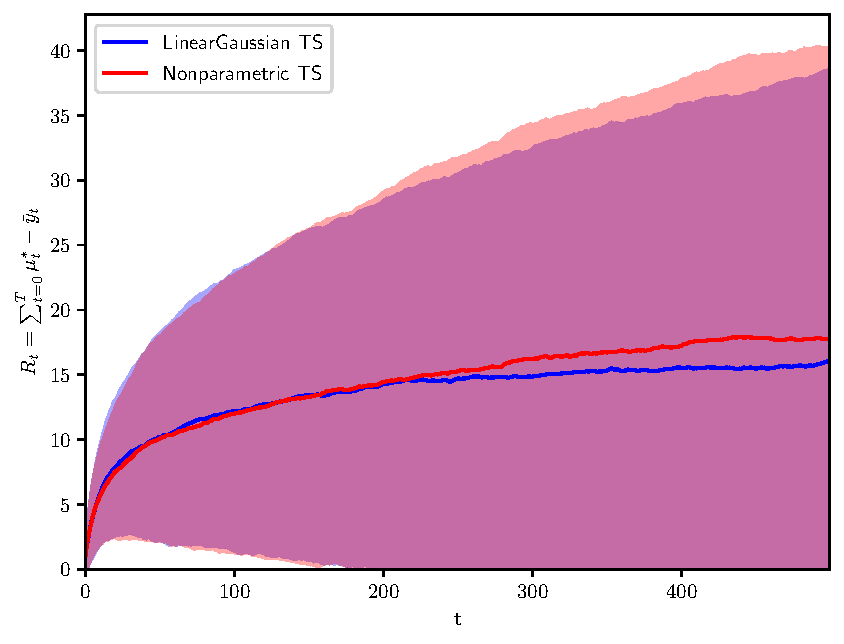
\includegraphics[width=\textwidth]{./figs/linearGaussian/cumregret_A2_-1_-1_1_1_1_1}
		\vspace*{-5ex}
		\caption{$|\mathcal{A}|=2$,\\ \hspace*{0.3cm}  $\theta_{0,i}=-1$, $\theta_{1,i}=1.0$.}
		\label{fig:linear_gaussian_A2_1}
	\end{subfigure}
	
	% A=3
	\begin{subfigure}[b]{0.32\textwidth}
		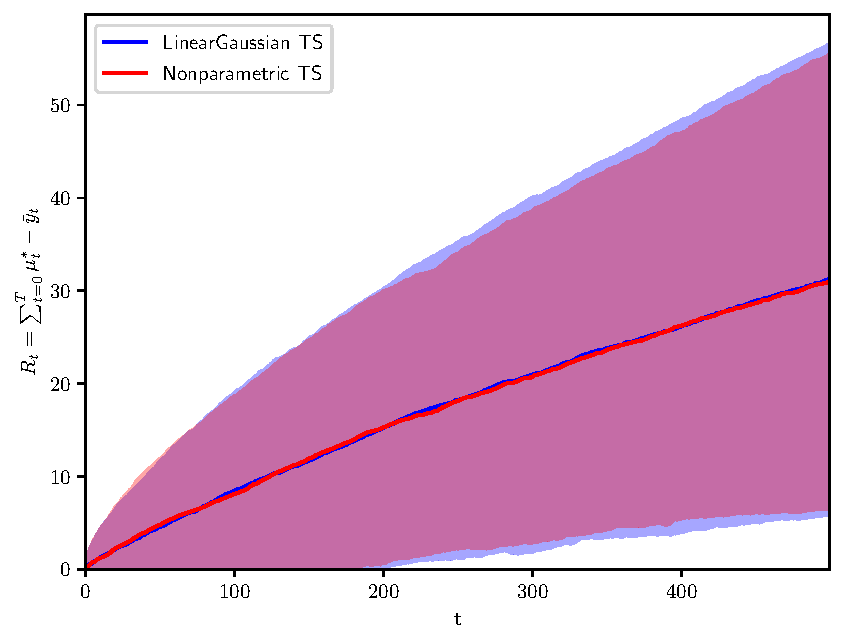
\includegraphics[width=\textwidth]{./figs/linearGaussian/cumregret_A3_-01_-01_0_0_01_01_1_1_1}
		\vspace*{-5ex}
		\caption{$|\mathcal{A}|=3, \theta_{0,i}=-0.1$, \\ \hspace*{0.3cm}$\theta_{0,i}=0, \theta_{2,i}=0.1$.}
		\label{fig:linear_gaussian_A3_01}
	\end{subfigure}
	\begin{subfigure}[b]{0.32\textwidth}
		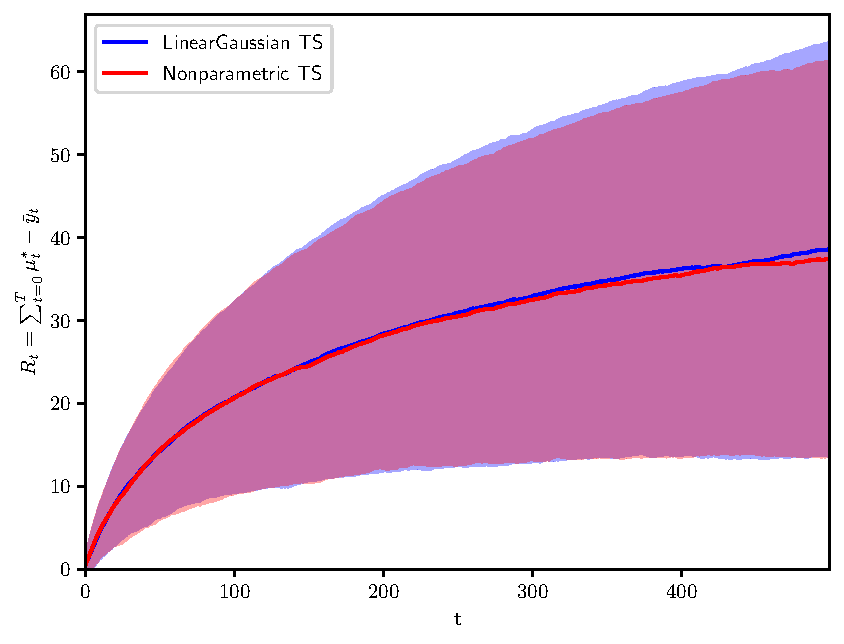
\includegraphics[width=\textwidth]{./figs/linearGaussian/cumregret_A3_-05_-05_0_0_05_05_1_1_1}
		\vspace*{-5ex}
		\caption{$|\mathcal{A}|=3, \theta_{0,i}=-0.5$, \\ \hspace*{0.3cm}$\theta_{1,i}=0, \theta_{2,i}=0.5$.}
		\label{fig:linear_gaussian_A3_05}
	\end{subfigure}
	\begin{subfigure}[b]{0.32\textwidth}
		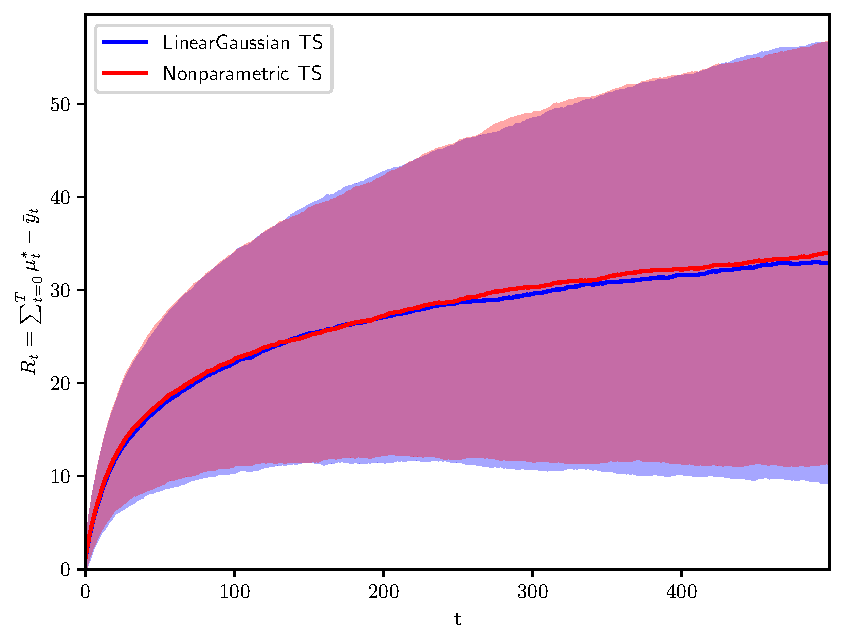
\includegraphics[width=\textwidth]{./figs/linearGaussian/cumregret_A3_-1_-1_0_0_1_1_1_1_1}
		\vspace*{-5ex}
		\caption{$|\mathcal{A}|=3, \theta_{0,i}=1$, \\ \hspace*{0.3cm}$\theta_{1,i}=0, \theta_{2,i}=1$.}
		\label{fig:linear_gaussian_A3_1}
	\end{subfigure}
	
	% A=4
	\begin{subfigure}[b]{0.32\textwidth}
		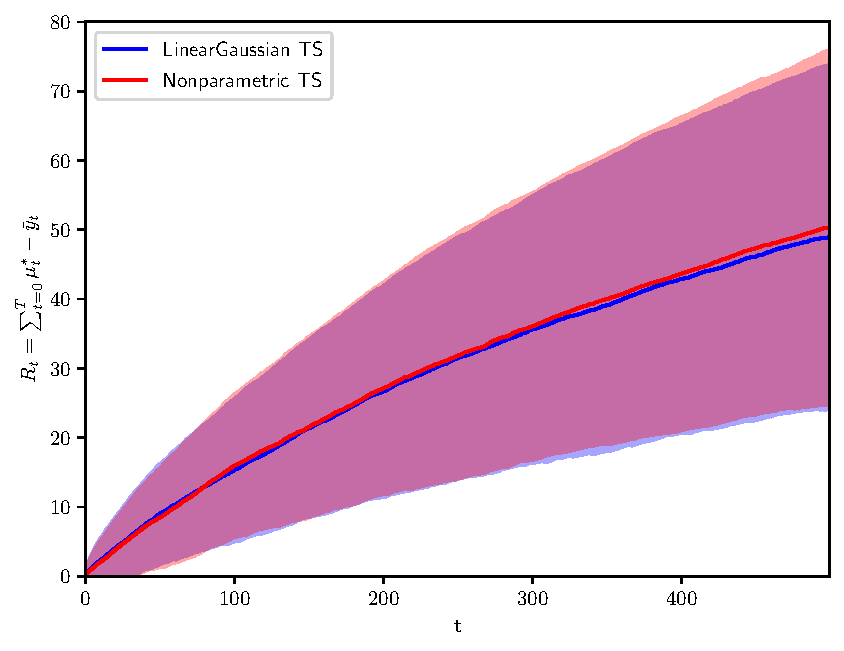
\includegraphics[width=\textwidth]{./figs/linearGaussian/cumregret_A4_-02_-02_-01_-01_01_01_02_02_1_1_1_1}
		\vspace*{-5ex}
		\caption{$|\mathcal{A}|=4, \theta_{0,i}=-0.2$,\\ \hspace*{0.3cm} $\theta_{1,i}=-0.1, \theta_{2,i}=0.1$,\\ \hspace*{0.3cm} $\theta_{3,i}=0.1$.}
		\label{fig:linear_gaussian_A4_01}
	\end{subfigure}
	\begin{subfigure}[b]{0.32\textwidth}
		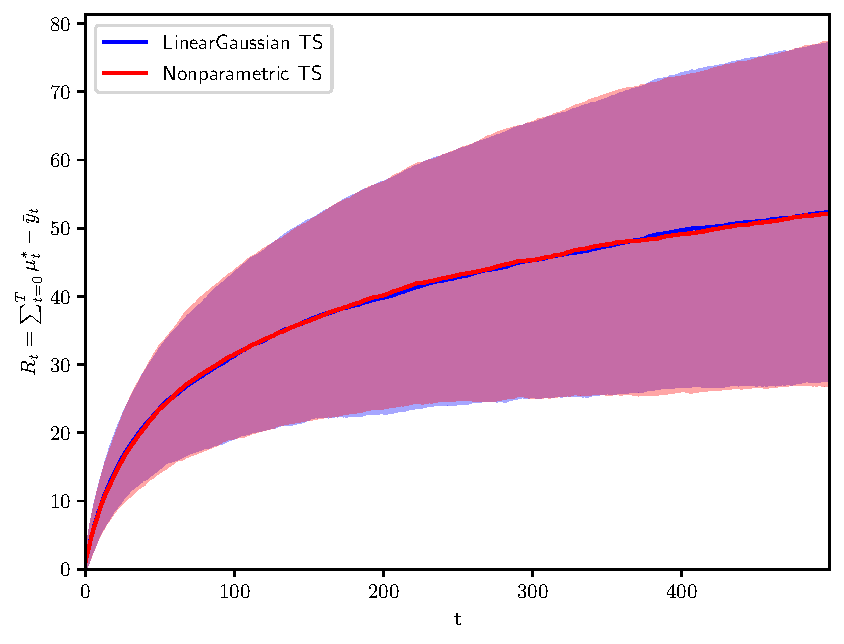
\includegraphics[width=\textwidth]{./figs/linearGaussian/cumregret_A4_-1_-1_-05_-05_05_05_1_1_1_1_1_1}
		\vspace*{-5ex}
		\caption{$|\mathcal{A}|=4, \theta_{0,i}=-1$,\\ \hspace*{0.3cm} $\theta_{1,i}=-0.5, \theta_{2,i}=0.5$,\\ \hspace*{0.3cm} $\theta_{3,i}=1$.}
		\label{fig:linear_gaussian_A4_05}
	\end{subfigure}
	\begin{subfigure}[b]{0.32\textwidth}
		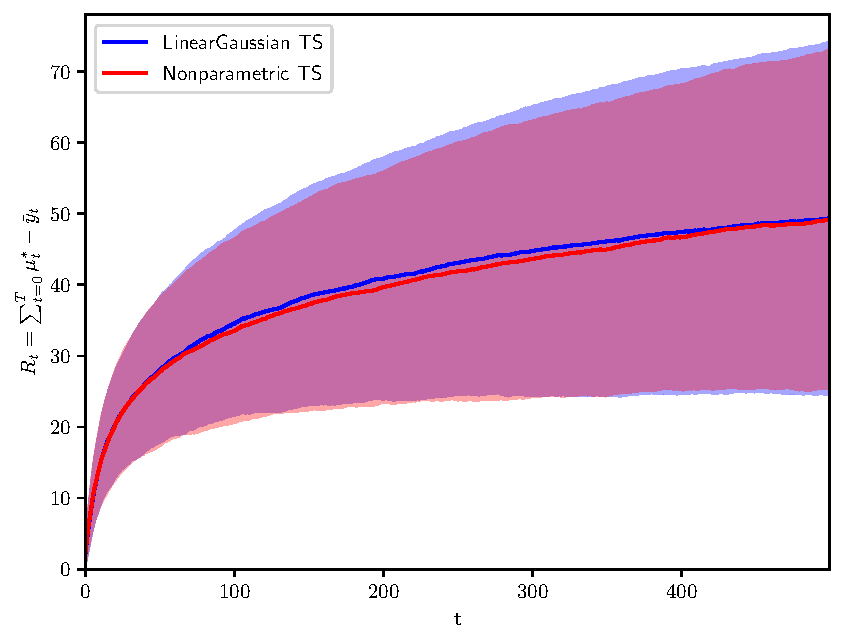
\includegraphics[width=\textwidth]{./figs/linearGaussian/cumregret_A4_-2_-2_-1_-1_1_1_2_2_1_1_1_1}
		\vspace*{-5ex}
		\caption{$|\mathcal{A}|=4, \theta_{0,i}=-2$,\\ \hspace*{0.3cm} $\theta_{1,i}=-1, \theta_{2,i}=1$,\\ \hspace*{0.3cm} $\theta_{3,i}=2$.}
		\label{fig:linear_gaussian_A4_1}
	\end{subfigure}
	
	\begin{subfigure}[b]{0.32\textwidth}
		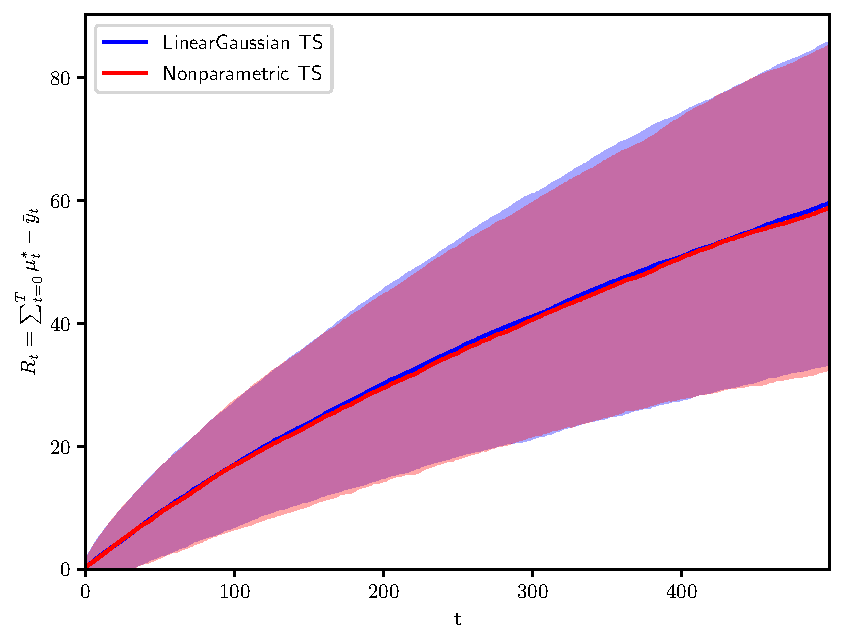
\includegraphics[width=\textwidth]{./figs/linearGaussian/cumregret_A5_-02_-02_-01_-01_0_0_01_01_02_02_1_1_1_1_1}
		\vspace*{-5ex}
		\caption{$|\mathcal{A}|=5, \theta_{0,i}=-0.2$,\\ \hspace*{0.3cm} $\theta_{1,i}=-0.1$, $\theta_{2,i}=0$,\\ \hspace*{0.3cm} $\theta_{3,i}=0.1, \theta_{4,i}=0.1$.}
		\label{fig:linear_gaussian_A5_01}
	\end{subfigure}
	\begin{subfigure}[b]{0.32\textwidth}
		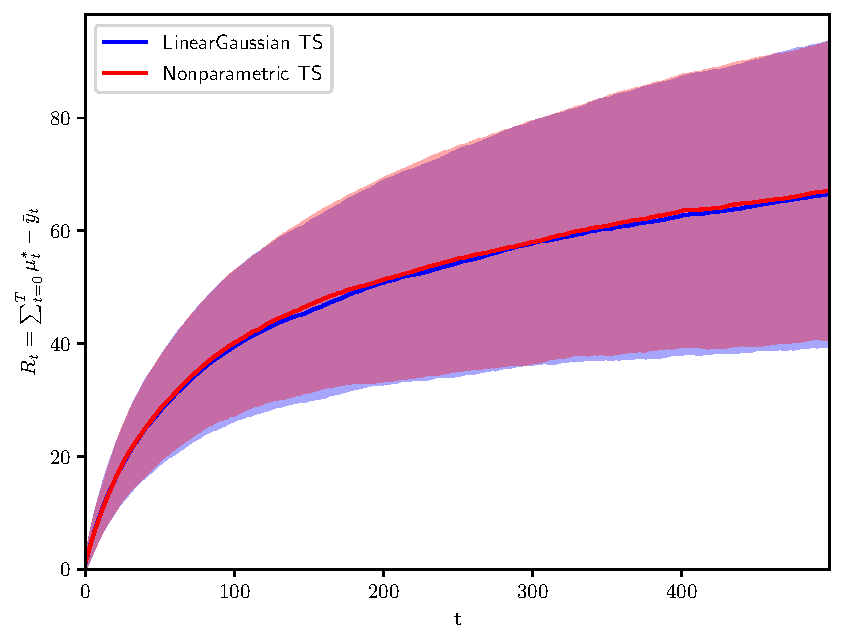
\includegraphics[width=\textwidth]{./figs/linearGaussian/cumregret_A5_-1_-1_-05_-05_0_0_05_05_1_1_1_1_1_1_1}
		\vspace*{-5ex}
		\caption{$|\mathcal{A}|=5, \theta_{0,i}=-1$,\\ \hspace*{0.3cm} $\theta_{1,i}=-0.5$, $\theta_{2,i}=0$,\\ \hspace*{0.3cm} $\theta_{3,i}=0.5, \theta_{4,i}=1$.}
		\label{fig:linear_gaussian_A5_05}
	\end{subfigure}
	\begin{subfigure}[b]{0.32\textwidth}
		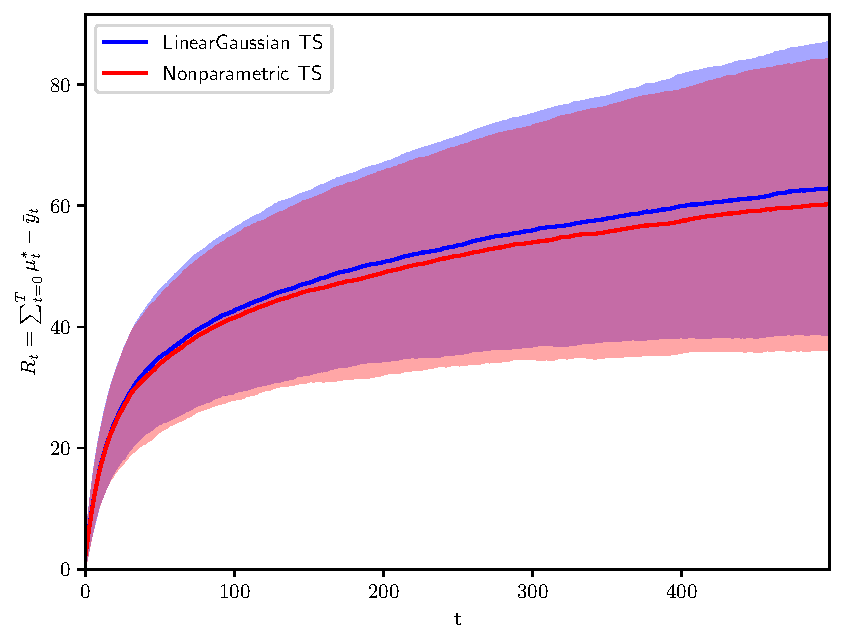
\includegraphics[width=\textwidth]{./figs/linearGaussian/cumregret_A5_-2_-2_-1_-1_0_0_1_1_2_2_1_1_1_1_1}
		\vspace*{-5ex}
		\caption{$|\mathcal{A}|=5, \theta_{0,i}=-2$,\\ \hspace*{0.3cm} $\theta_{1,i}=-1$, $\theta_{2,i}=0$,\\ \hspace*{0.3cm} $\theta_{3,i}=1, \theta_{4,i}=2$.}
		\label{fig:linear_gaussian_A5_1}
	\end{subfigure}
	%\vspace*{-2ex}
	\caption{Mean cumulative regret (and standard deviation shown as shaded region) for $R=1000$ realizations of different $\A=\{2,3,4,5\}$ armed contextual linear Gaussian bandits, with $\sigma_a^2=1 \forall a$.}
	\label{fig:linear_gaussian_oracle}
	%\vspace*{-4ex}
\end{figure*}

We showcase the flexibility of our proposed method in the contextual linear Gaussian MAB setting first, where we can readily compare its performance to a well studied \texttt{Oracle TS}: \ie the linear Gaussian Thompson sampling in~\cite{ip-Agrawal2013a}.
In this set-up, \texttt{LinearGaussian TS} correctly assumes the true underlying contextual linear Gaussian model $Y_{t,a}\sim \N{Y|x_t^\top\theta_a, \sigma_a^2}$, and can compute posterior updates in closed form. 

In Figure~\ref{fig:linear_gaussian_oracle}, we show the mean cumulative regret of various parameterizations of multi-armed ($\A=\{2,3,4,5\}$) contextual linear Gaussian bandits, with two-dimensional contexts randomly drawn from a uniform distribution, \ie $x_{i,t}\sim\U{0,1}$, $i\in\{0,1\}$, $t\in \Natural$.

The proposed \texttt{Nonparametric TS} attains cumulative regret comparable to that of \texttt{LinearGaussian TS}. 
That is, the proposed method matches the performance of the analytical linear Gaussian posterior Thompson sampling, even as it estimates the true form of the underlying reward function.

The proposed nonparametric Thompson sampling is almost as good as the analytical alternative when there is no model mismatch, as in this setting: the per-arm nonparametric posterior density quickly converges to the true unknown distribution, incurring in minimal additional regret when compared to the analytical posterior based \texttt{Oracle TS} alternative.